\documentclass[a4paper,11pt]{article}

\usepackage{float}
\usepackage{graphicx}
\graphicspath{./Diagrams}
\setlength{\oddsidemargin}{0in}
\setlength{\evensidemargin}{0in}
\setlength{\textwidth}{160mm}
\setlength{\topmargin}{-15mm}
\setlength{\textheight}{240mm}


\begin{document}
\section{Design}
For the overall design of for the solver experiment code can be split into, the solving algorithms, and the sudoku puzzles representation. There will be two different versions of the solver, which have common features, can use object oriented principle of inheritance which will also help at the later on stages of the experiment code, using polymorphism. The collection of puzzles(population) will also be an attribute in the solver class.

\subsection{Requirements}

Load sudoku puzzles from a file\newline
For the Hybrid repair algorithm:
\begin{itemize}
	\item Solve a 4x4 puzzle  
	\item Solve a 9x9 puzzle
\end{itemize}
For the Multi-objective algorithm:
\begin{itemize}
	\item Solve 4x4 puzzle
	\item Solve 9x9 puzzle
\end{itemize}
Perform experiments on sets of example sudoku:
\begin{itemize}
	\item For 4x4 puzzle
	\item For Easy 9x9 puzzles
	\item For Medium 9x9 puzzles
	\item For Hard 9x9 puzzles
	\item For Expert 9x9 puzzles
\end{itemize}



\subsection{Representation of Sudoku Puzzle}
Representing the puzzle within the program was a key issues within its creation. The representation used within this program is rather simple, for any space that has a integer value, it uses that integer, e.g. for a 9x9 puzzle it could be any number between 1 and 9. However the issues of blank spaces when trying to solve the program still remains, to deal with this I have extended the range to 0-9, where 0 represents a blank space and 1-9 represents 1-9. The integers for the puzzle are stored in a 2D array, looking very similar to an actual sudoku puzzle, as seen in figure 2. Due to the simplicity of the representation, it also comes with some notable issues. Namely the size of the search space that this creates for the algorithm, especially as the size of the puzzle increases. 
\begin{figure}[h]
	\caption{Representation for encoding of sudoku puzzle}
	\centering
	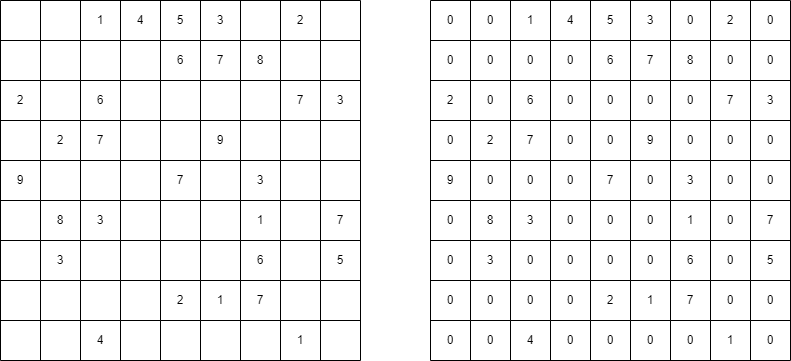
\includegraphics[height=4.5cm, width=10cm]{./Diagrams/representationDiagram}
\end{figure}



\subsection{Puzzle class}
The puzzle class, needs to store the state of the puzzle being solved and the fitness value of the puzzle. The state of the puzzle as previously detailed will be stored in a 2D array of int, the fitness value(s) should be stored in an array of variable size, this allows the puzzle to be set for either type of solver allowing for either single or multi-objective fitness functions. There are two different constructor methods for the puzzle class, a normal constructor and a constructor for copying puzzles. The normal constructor needs the size of the puzzle, the initial puzzle state and number of objectives the fitness function, used to define of the size of the fitness array.\newline \newline The most important methods outside of the setters and getters, are the methods used to find rule violations and empty spaces. The violation finder method, is important for adding rules, where it is used in the repair method as a way to apply the rules of the game to solver and also used as a part of the fitness function for multi-objective. The method is split into several smaller steps, finding each violation for the 3 different rule violations, counting the number of constraint violations each space in the puzzle has and sorting the spaces with violations by number of violations.\newline \newline Finding the constraint violations for the row and column, loops through each space in the row or column and comparing the value to each other space on the board. Counting the grid violations is a similar process, however it has to go through the individual grid, which uses a messier loop. The issues with this way of counting violations, is that it counts each violation twice. The empty spaces algorithm, should return an array of all locations within the puzzle space, that have a 0 value, which is useful for the fitness functions and seeing if the puzzle is complete.

\subsection{Solver Class}

The Solver class is the parent class for the two different types of EA being used in the experiment, so stores their common features, the attributes in the class are, the population which is an ArrayList of puzzle objects, and the initial state of the puzzle which is an array that holds the initial state of the puzzle. The important methods that are used by both solvers, are generating the population, mutation of the individual puzzles, checks for whether the puzzle is complete, a space is part of the initial puzzle and finally a method for loading the initial puzzle from a file.  \newline\newline Generating the intial puzzle, is a simple algorithm, that takes a puzzle, creates the initial state from that puzzle, find the fitness value for the puzzle, then adds mutations of the initial puzzle with updated fitness values, to the population, until the defined size of the population is reached. \newline\newline Mutating a puzzle, displays a different behaviour based on the state of the puzzle. If the puzzle still has empty spaces, it adds a random number between 1 and the puzzle size, to a random empty space in the puzzle. The alternative behaviour is for where all the spaces in the puzzle have been filled, but the puzzle is not yet complete, which only happens to the multi-objective solver, as the repair method for the hybrid solver will always remove values that are violation before mutation happens again. For the alterative behaviour, the mutation changes a random space, that is not in the initial configuration, to a random value between 1 and the puzzle size.\newline\newline The method that checks puzzles completion, looks at every puzzle in the population, if for that puzzle, there are no constraint violations and no empty spaces, meaning the puzzle is full and none of the rules of sudoku have been violated. If a puzzle that meets these conditions is found, the method prints the puzzles state and returns true, if no completed puzzle is found the method returns false. \newline\newline Loading a puzzle from a file is needed in the experiment, the method takes a file path and the puzzle size and simply uses a scanner to read from the file, until there required number of ints are taken for the puzzle size, this does require that the files provided do not use any illegal numbers, outside the range of the puzzle, however given that the this method is only being used specifically for an experiment with files created specifically for that purpose, there is no need to deal with illegal cases. 

\subsection{RepairBasedSolver class}

The RepairBasedSolver class is an implementation of the hybrid repair based EA and is used in the experiment to review the algorithm.\newline\newline The class extends the solver class and only adds 7 unique methods:
\begin{itemize}
	\item getSolution
	\item mutatePopulation
	\item sortPopulation
	\item splitPopulation
	\item repairPuzzle
	\item repairPopulation
	\item updateFitness
\end{itemize}
The getSolution method is the most important method in the class, is an implementation of the EA itself, as detailed in chapter 2.3. Taking a puzzle, the method, generates the population for the algorithm, creates a counter and while loop which checks if the puzzle is completed and the counter has not surpassed the maximum number of generations. Inside the while loop, the counter increases, then the population is repaired, this order changes from figure ?, due to the way the population is generated, as each member is mutated once, meaning many individuals will have have broken the rules, which means without the repair happening before more feasible individuals would be taken out by the selection algorithm. The sort then takes place, with the splitPopulation afterwards before finally mutating and going back to the loop conditions, once the loop has finished the population is cleared and the number of generations taken is returned. \newline\newline The mutation of the population, for each member of the population, creates a copy of the puzzle, mutates and updates the fitness values of both the parent and child puzzle object, then adds the children to the population.\newline\newline The sortPopulation is a method that takes the population and sorts them based on their fitness values. The splitPopulation method acts is the selection algorithm and is rather simple. It removes half the population, by using the sortPopulation all it has to do is remove the front half of the ArrayList. \newline\newline The repairPuzzle method takes the list of violations from the puzzle object, and removes any conflicting space that is not permanent. The repairPopulation method just goes through each member of the population, and loops until the puzzle being looked at is feasible by calling the repairPuzzle method. The updateFitness method takes the roll of the fitness function in this solver class, the fitness calculation is simple, taking the total number of filled spaces as the fitness.

\subsection{Multi-objective class}
The MultiObjectiveSolver class is an implementation of the multi-objective EA and  is used the experiment as one of the two EA being compared.\\\\ It extends the solver class and has 5 methods and a new attribute:
\begin{itemize}
\item mutatedPopulation
\item getSolution
\item mutatePopulation
\item splitPopulation
\item compareFitness
\item updateFitness
\end{itemize}

Mutated population is a field exclusive to the MultiObjectiveSolver class, t is an ArrayList of puzzles which is used to temporarily store puzzles during the mutatePopulation and splitPopulation methods.\\\\ The getSolution method, is the implementation of the EA itself, detailed in chapter 2.4. Taking a puzzle, a population is generated, after this algorithm initiates a counter, used to monitor the number of generations gone through. A while loop, with the conditions to exit the loop being the counter surpassing the maximum number of generations or the puzzle being completed. Inside the loop each time the counter is increased by one. The population then mutates, updates its fitness values and then performs selection on the population. Once one of the exit conditions is satisfied and the loop is exited, the population is cleared, and the number of generations taken is returned. \\\\ The mutatePopulation method, creates a child for each puzzle in the population, these children are added to the mutatedPopulation field, where mutatePuzzle is then used on each of them, and their populations are also updated.\\\\ The splitPopulation method used to represent the selection in the EAs, uses the compareFitness method to compare the fitness of the parent and mutated children puzzle, if the child puzzles fitness values surpasses the parent, it replaces the parent in the main population ArrayList, otherwise the parent stays. Once every member of the population is compared, the mutated population is the then made null.\\\\ The compareFitness function is a helper function used by splitPopulation, it takes two puzzles and compares both of their fitness values, returning true if the first puzzle is greater and false otherwise. The updateFitness method, finds the number of filled spaces and the number of violations that exist.  

\begin{figure}[h]
	\caption{Class diagram for the program}
	\centering
	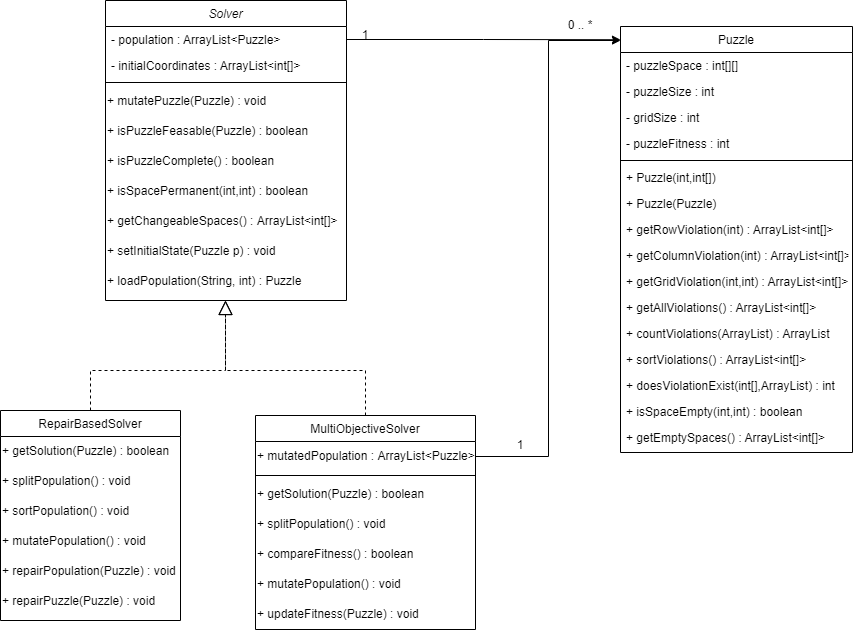
\includegraphics[height=15cm,width=18cm]{./Diagrams/classDiagram}
\end{figure}

\subsection{Experiment program }
The experiments will be done in two steps, the first being collecting data concerning failures and number of generations from the two algorithms performance on a set of sudoku puzzles of different size and difficulty, which will be done in Java. The second step is putting that data in R using scripts and getting greater insights on the results, via graphs and statistical tests.\\ The experiment in Java, will test a solver against 10 puzzle files of some size or difficulty , produce a report of the number of generations and time taken for that attempt. A seperate file will store a report of the average, number of generation(excluding failures), number of failures and time taken. By doing this for all the puzzle sizes and difficulties provided, the data can then be analysed and used for the conclusions. The Java experiment program itself, should for a solver, then for each puzzle, load the puzzle into the solver, and attempt to solve the puzzle 30 times, producing the results detailed earlier and writing them to a file.    


\end{document}


